\documentclass[10pt]{report}
\usepackage[utf8]{inputenc}
\usepackage[italian]{babel}
\usepackage{multicol}
\usepackage[bookmarks]{hyperref}
\usepackage[a4paper, total={18cm, 25cm}]{geometry}
\usepackage{graphicx}
\usepackage{xcolor}
\usepackage{textcomp}
\graphicspath{ {./img/} }
\usepackage{listings}
\usepackage{makecell}
\lstdefinestyle{customasm}{
  belowcaptionskip=1\baselineskip,
  frame=line,
  xleftmargin=\parindent,
  language=[x86masm]Assembler,
  basicstyle=\ttfamily,
  commentstyle=\itshape\color{purple!40!black},
}
\lstset{escapechar=@,style=customasm}
\lstnewenvironment{C}
  {\lstset{language=C++,frame=none}}
  {}
\begin{document}
\title{Algorithm Engineering}
\author{Federico Matteoni}
\date{A.A. 2021/22}
\renewcommand*\contentsname{Index}

\maketitle
\begin{multicols}{2}
\tableofcontents
\end{multicols}
\pagebreak
\section{Introduction}
Teacher: Paolo Ferragina\\
Exam: written + oral. Midterms in November and December, with exercises.\\
Classes will be recorded on Microsoft Teams. Also the book "The Magic of Algorithms" is very important: you must be used to talk about these things, not just be able to solve exercises.
\paragraph{Course} \textbf{Design} and \textbf{analysis} of algorithms but also insights about \textbf{implementation}, with reference to libraries and considerations about what happens when using certain algorithms. The case of use is \textbf{big data}.
\paragraph{Algorithm} Knuth's definition: "\textit{a finite, definite, effective procedure that takes some input and returns an output, with the output being the answer to the problem you want to solve}." So, a finite sequence of steps, not only a finite numbers of operations but also the algorithms must \textbf{terminate}. \texttt{while (true) do ...} will go on forever, so it's not an algorithm. Definite means that the steps are definite in an unambiguous way. Effective means that every step is basic, atomic, something that we can execute in small or constant time, constant is not a very precise word (seconds? Milliseconds?) so we will accept the "small time" rough definition. Also, the mapping input $\rightarrow$ output must always be correct, which is the biggest difference with IA. An algorithm outputs the correct output for each input.
\paragraph{RAM} Random Access Machine, CPU $\leftrightarrow$ M, classical computing model (Von Neumann machine), the memory can read any place in constant time.\\
We will make a more sophisticated step. But without presenting very complicated models. We need a good balance, not perfect but a better approximation than the RAM.
\paragraph{} Algorithm A and find function $T_A(n)$ that describes the time complexity of A. $n = $ input size, number of items that the algorithm has to process. Hours, seconds, milliseconds based on the machine, but we approximate the time taken with the number of steps. Also, the number of steps depends on the number of items but also on the items themselves. So we usually analyze the worst case scenario, or less often the average scenario. Analyzing the worst case scenario we can figure out the worst or "maximum" number of steps. \textbf{Asymptotic analysis}.\\
We want to exploit the characteristics of the various types of memory.\\\\
We will count not steps but the I/O ops, with a 2 level memory model: the first model is the internal fast memory (cache + RAM) and the second level is the mass memory (disk). In small memory situations, the first level can be interpreted as cache and the second level as internal memory, other times the first level is the internal memory and the second level is unbound slow memory.
\begin{list}{}{}
	\item Spatial Locality: access near items
	\item Temporal Locality, or small working set: far apart items used often so we can exploit their presence in the cache
\end{list}
\paragraph{Poly vs Exp time complexity} Let's say we have three algorithms: $n$, $n^2$, $2^n$ in time complexity respectively. Let's express the time complexity fixing $t$ time and counting how many items we can process in $t$ time. In the first case is linear, so $n = t$, the second is $n = \sqrt{t}$ and the third is $n = \log_2 t$. If we have a $k$ times faster machine, we can imagine using the original machine for $k$ more times. $n = kt, n = \sqrt{kt}, n = \log_s kt$. The linear algorithm has full advantage of the $k$ times faster machine, the second algorithm has a small advantage of a multiplication factor $\sqrt{k}$ and the last a negligible advantage of a sum factor of $\log_2 k$, which is basically none.
\paragraph{Analysis} $A[1, n]$ integer array of which we want to compute the sum. The number of steps is $n$.\\
First situation: first we load $B$ items and process thems, then the next $B$ items $\Rightarrow$ \# I/O = $n/B$, which we will see often and is called the \textbf{scan cost}, because we need to see each element, in batches of $B$ elements. So $B$ is the size of the memory page.\\
But we can follow a different approach: we take the first item of each batch of $B$ elements, then the second items and so on, which will take $n$ steps, but this will be possibly slower because this method takes more I/Os ops, $n$ I/O ops. The larger the jumps the more I/O ops we do. The model doesn't distinguish between local and random I/Os.
\paragraph{Binary Search} Array of $n$ elements. We pick the middle element, we go to left/right, middle element of the section and so on. The time complexity is $T(n) = O(\log_2 n)$, but we have a lot of I/Os and big jumps, so elements in different and far pages. We have $log_2 n/B$, because at a certain point the subarray where we search is smaller than a page, so we have $\log_2 n$ steps $- \log_2 B$ the last steps inside the page, and for the properties of the logarithms we have $\log_2 n/B$. So the larger the page the smaller the number of I/Os.  One consideration: $n$ is the number of items, $B$ is in kilobytes. So if we consider integers of 8 bytes, we have $B/$size items, and with $B =$ 32 kb = $2^{15}$ kb we have circa 4000 times, or $2^{15}/2^3 = 2^{12}$.\\
How can we improve the search? We can consider the $B^+$-trees. We split the array into the page size $B$ and the array is sorted in ascendent order. The splits are called leaves, and each leaf has a key (one of the elements). We have a page with each key and the next element is the pointer to its page. Above one level, a page with a key of the first key list and a pointer to the key list, a key of the second and so on.\\ %numero di elementi da rivedere
Fetch a page, binary search and follow the pointer. Number of I/Os is $\log_B n/B$ and the number of steps is a binary search for every page, so $(\log_B n/B)$ pages $\cdot \log_2 B$
\paragraph{Analysis}
$n = (1 + \epsilon)M$ with $\epsilon > 0$ data outside of the memory. So $M$ is totally full and $\epsilon M$ is stored in the unbound memory.\\
The first point is we want to find $P($accessing the disk$)$, with a totally random algorithm, is $= \frac{\epsilon M}{n} = \frac{\epsilon\not M}{(1 + \epsilon)\not M} = P(\epsilon)$\\\\
The second point is the average time of a step. $\sum_x P(X = x)\cdot x$ with $X$ the variable of which we compute the average with that formula. $X$ is time, in this case. The time is $1$ in case of computing, and varies in case of accessing the memory. So we have the multiply the cost of access times the probability (of computing, going internal, going to the disk). Internal memory access costs 1, while on disk is larger and we say that the cost is $c$. So the average, with let's say $a$ probability of memory access, $= (1 - a)\cdot 1 + a(P(\epsilon)\cdot c + (1 - P(\epsilon))\cdot 1)$ but $0 < a < 1$ and $1 - P(\epsilon)$ are very small, so we can rewrite as $= a\cdot P(\epsilon)\cdot c = a \cdot \frac{\epsilon}{1 + \epsilon} \cdot c + O(1)$. If $a = 0$ then no memory access so the cost is constant. The larger is $a$ the more memory access, the more the term is important, which is exactly what we want to capture. Usually, $a = 0.3 = 30\%$ and $c = 10^6$ the gap between accessing the disk and accessing the internal memory.\\
So $\frac{\epsilon}{1 + \epsilon}\cdot 0.3 \cdot 10^6 = \frac{\epsilon}{1 + \epsilon} \cdot 300000$. If $P(\epsilon) = 0.001$ the avg time of a step is $0.001 \cdot 300000 = 300$, so the disk has a lot of impact even with only a thousandth of memory access being on disk: the avg cost is 300 and not 1.
\paragraph{Sorting and permuting} Given an array $S[1, m]$ and a permutation $\pi$, the permutation problem asks to permute $S$ according to $\pi$. For example $S = [A, B, C, D], \pi = [3, 1, 2, 4]$ then $\pi$ tells that the $\pi[0] = 3$ item goes to the first position. So $S_\pi = [C, A, B, D]$.
\begin{lstlisting}
for i = 1 to n:
	S'[i]=S[pi[i]]
\end{lstlisting}
Which costs $\Theta(n)$\\
\begin{tabular}{c | c | c}
 & PERM & SORT \\
\hline
RAM & $n$ & $n\log n$\\
\hline
2-level memory & min\{$n$, $C_{sort}$\} & $C_{sort}$
\end{tabular}\\
Solving the permuting in a scan + sort kind of way, -altrimenti- we have to do a disk access per value.\\
\begin{list}{}{}
	\item scan S : $\langle$S[i], i$\rangle$ which is $\langle$item, position$\rangle$\\
	Which creates $\langle$A, 1$\rangle$ $\langle$B, 2$\rangle$ $\langle$C, 3$\rangle$ $\langle$D, 4$\rangle$\\
	This costs $O(n/B)$
	\item scan $\pi$ : $\langle\pi$[i], i$\rangle$ which is $\langle$src, dst$\rangle$\\
	Which creates $\langle$3, 1$\rangle$ $\langle$1, 2$\rangle$ $\langle$2, 3$\rangle$ $\langle$4, 4$\rangle$\\
	This costs $O(n/B)$
	\item sort by first component of the sequence $\langle\pi$[i], i$\rangle$\\
	Which creates $\langle$1, 2$\rangle$ $\langle$2, 3$\rangle$ $\langle$3, 1$\rangle$ $\langle$4, 4$\rangle$\\
	We take the item in source and move to destination
	\item parallel scan
	$\langle$A, 1$\rangle$ $\langle$B, 2$\rangle$ $\langle$C, 3$\rangle$ $\langle$D, 4$\rangle$\\
	$\langle$1, 2$\rangle$ $\langle$2, 3$\rangle$ $\langle$3, 1$\rangle$ $\langle$4, 4$\rangle$\\
	Which creates $\langle$A, 2$\rangle$ $\langle$B, 3$\rangle$ $\langle$C, 1$\rangle$ $\langle$D, 4$\rangle$\\
	\item sort by second component\\
	Which creates $\langle$C, 1$\rangle$ $\langle$A, 2$\rangle$ $\langle$B, 3$\rangle$ $\langle$D, 4$\rangle$\\
	\item scan\\
	Which creates [C, A, B, B]\\
	This costs $O(n/B)$
\end{list}
The I/O cost is 4 scan + 2 sort $= O(\frac{n}{B}) + 2\cdot O(C_{sort})$ sorting cannot cost less than $\frac{n}{B}$ because we can't improve that, so $O(C_{sort})$\\\\
So we have proposed upper-bounds = algorithms for the sorting and the permuting problem. The permuting problem can be solved in $O(\frac{n}{B}) +$ sorting I/Os. Moving $n$ items takes $\Theta(n)$ I/Os.\\
Sorting $n$ items in a two level memory of size $M$ for internal memory and $B$ for the disk page size, costs $O(\frac{n}{B} \cdot \log_{\frac{M}{B}} \frac{n}{M})$ with $L = \log_{\frac{M}{B}} \frac{n}{M}$, and often written as $\overline{O}(\frac{n}{B})$ with the overline or over tilde that means that is a scan.\\
$L$ consists of the base $\frac{M}{B}$ and the argument $\frac{n}{B}$ which means that with a larger memory I'd like it to be faster, with bigger $M$ the argument decreases and the base increases so the logarithm shrinks a lot. With a bigger $B$ page size, $\frac{n}{B}$ decreases but the base increases.\\
$\frac{M}{B} =$ how many pages I can keep in the internal memory. Let's say $n = 2^{40}$, $M = 8$Gb $= 2^{33}$ and $B = 32$Kb $= 2^{15}$, then $$\log_{\frac{n}{B}} \frac{n}{M} = \frac{\log_2\frac{n}{M}}{\log_2 \frac{M}{B}} = \frac{\log_2 \frac{2^{40}}{2^{33}}}{\log_2 \frac{2^{33}}{2^{15}}} = \frac{\log_2 2^7}{\log_2 2^{18}} = \frac{7}{18} < 1$$
Let's see when is sorting preferred to moving items or viceversa
$$\frac{n}{B} \log_{\frac{M}{B}} \frac{n}{M} < n \Leftrightarrow \log_{\frac{M}{B}} \frac{n}{M} < B$$\\
We have $B = 1$ in the RAM model, $B = 32$Kb in the 2-level model compared to $\log_{\frac{M}{B}}\frac{n}{M} = 2$ or $3$. In practical situations with disk, sorting is better than moving numbers. If $B = 1$, in the RAM model, $M = O(1)$, then sorting is worse than moving.
\paragraph{Sorting} Let's consider binary merge sort, which in the worst case costs $O(n\cdot \log_2 n)$. Let's evaluate the I/Os in the case that $n >> M$ so the array can't be stored entirely in internal memory. Since it's based on the merge procedure, we can evaluate the cost of the merge and multiply by the number of levels. It loads a page every time it needs it and writes a pages every time it fills one. So if the two arrays to merge are long $l$, it makes $\frac{l}{B}$ I/Os. So it takes $O(\frac{n}{B} \log_2 n)$ I/Os.\\
Sorting = computing the sorted permutation + implement the sorted permutation. So we can say that sorting $\geq$ permuting, is at least difficult as\ldots. In the RAM model the $\geq$ is $>$, strict, because sorting is $n\cdot\log n$ and computing is the real issue, because implement is linear. In the 2-level memory model they are almost equivalent. This considering \textbf{atomic items}, integers o non-splittable strings.\\
The mismatch is the base of the logarithm. The binary merge sort is $O(\frac{n}{B} \log_2 \frac{n}{M})$: partitioning the array in blocks of size $M$, the size of the memory, called runs. Can we generate runs longer than M in few I/Os? On average we will be able to create runs of size $2M$, which saves 1 full scan of data (which, for large data, is a lot of time saved).
\paragraph{Snow plow algorithm} Sort item that you can, leave item that you cannot.\\
S = 1, 7, 5, 3, 2, with M = 3 items. The memory is divided in two parts: a min heap, items that are still unsorted, and an unsorted part, the snow that we cannot clean. Start from the memory with everything unsorted: min heap empty and only unsorted items. We put $M$ unsorted items, so 1, 7, 5 in the unsorted part. We sort the unsorted items and move to the min heap, with the unsorted part left empty. We pick the minimum element and write it out of the memory. We have emptied a position, and we can fetch another item in the unsorted part, the 3. The new item is compared to the minimum. 3 is larger than the current minimum, so is written inside the min heap, which is now 3, 5, 7. We write again out the minimum, 3, and fetch another item. 2 is smaller than 3, so it goes in the unsorted part. At some point the min heap will be empty, the unsorted part will be full and we restart the phase. We pay 1 I/O as soon as we write out $B$ items.
\begin{center}
	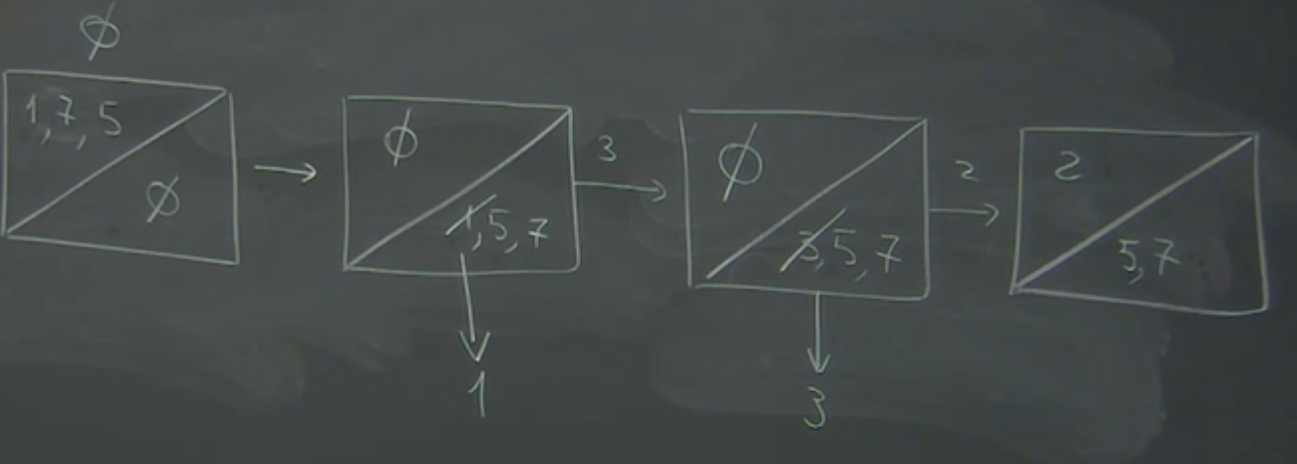
\includegraphics[scale=0.5]{1.png}
\end{center}
Let's prove that the runs are 2M on average. We start with $|U| = M$ and $|H| = 0$, with U unsorted part and H heap part. Continuing we read items, with $T = \#$ items read. The phase has processed $T + M$ items, $T$ read and $M$ already in memory. At the end of the phase, the min heap is empty $|H| = 0$ and $|U| = M$ and $T$ items are written out. So $T$ is the length of the run, we have to compute it, by making hypothesis about the distribution of the items, the probabilities of going to U and H. P(item read goes to $U$) = $1/2$, a totally random situation. By changing the probability we change how much sorted is the sequence. The more sorted is the sequence, the smaller the probability of going to $U$. avg$(|U|) = E[|U|] = T/2$. Given that $|U| = M$, then on average $E[|U|] = \frac{T}{2} = M$ so average $T = 2M$
\paragraph{Exercise} $M = 2$ and $S = 1, 8, 3, 2, 5, 0, 4, 6$\ldots
\paragraph{Issues} Binary Mergesort doesn't always exploit all the memory. Because after creating the $M$-long first runs, by merging we need $3B$ for reading the memory (one for the first run, one on the second run and one page on the output), so $3B << M$, a lot of unused memory. We could fetch 2 pages per run, but the second page can be used only after the first page, so no advantage in allocating all data. Since there's a sequence of processing, even if a load immediately all the pages, we do not have much advantage in doing so. So we would like to merge $k$ runs instead of two runs at a time. Since we want to fill the memory, we want $(k+1)B = M$, $k$ pages for $k$ runs plus an output page. So $k = \frac{M}{B} - 1$ which we can approximate with $\frac{M}{B}$. Each run generates $l/B$ I/Os, and the merged run is long $kl$ elements.\\
So every run is of $M$ elements which take $\frac{M}{B}$ I/Os, for $n/M$ runs. So the total cost is $O(n/M \cdot \frac{M}{B}) = O(n/B)$ for creating runs. ?So $\log_k n/M$?.\\
The cost of mergesort is $O(n/B + n/B\cdot\log_k n/M)$ which we have seen with $k = \frac{M}{B}$.\\
With improve B, M by compression. So 3, 5, 10 is written as 3 (the first item) and storing the gaps (gap encoding) so 2, 5,\ldots with variable length encoders.\\\\
Let's rewrite the bound
$$\frac{n}{B}\cdot\log_{\frac{M}{B}}\frac{n}{M}$$
We don't know how items are consumed on the disks, given $D$ disks. With $k = 2, D = 2$ we can take advantage of the parallelism on the first load. But once loaded in memory, we may consume the pages asymmetrically, so we may end up reading a lot from a disk and very few times from the other. Possibly, every page on the first disk is used before the second page on the second disk. So by adding more disks we take full advantage because they are the denominators. The know optimal bound is:
$$\Theta\left(\frac{n}{BD}\cdot\log_{\frac{M}{B}}\frac{n}{BD}\right)$$
For 1 disk is $O(\frac{n}{B}\cdot\log_{\frac{M}{B}}\frac{n}{B})$\\
For $D$ disks we can consider one big disk with $B' = D\cdot B$ page size, so the heads of the disks are fixed together and move together. We do not change the algorithm, so the complexity is simply $O(\frac{n}{B'}\cdot\log_{\frac{M}{B'}}\frac{n}{B}) = O(\frac{n}{DB}\cdot\log_{\frac{M}{DB}}\frac{n}{DB})$ but with D in the base of the logarithm makes the value larger, but the impact is small and the simplicity of the method makes it worth it. This is called \textbf{disk striping}.
\paragraph{Binary Decision Trees} The leaves there are permutations.
\end{document}